\documentclass[border=6pt]{standalone}
\usepackage{tikz}
\usepackage{pgfplots}
\pgfplotsset{compat=1.18}
\usetikzlibrary{arrows.meta,positioning,shapes.geometric,fit,backgrounds,calc,decorations.pathreplacing,patterns,pgfplots.groupplots}
\tikzset{
  blk/.style={rectangle, rounded corners=2pt, draw=black!70, thick, fill=blue!6,
              minimum height=8mm, minimum width=20mm, align=center, font=\small},
  io/.style={rectangle, rounded corners=6pt, draw=black!70, thick, fill=green!8,
             minimum height=8mm, align=center, font=\small},
  proc/.style={rectangle, draw=black!70, thick, fill=orange!10, minimum height=8mm,
               align=center, font=\small},
  dec/.style={diamond, aspect=2, draw=black!70, thick, fill=yellow!15, align=center, font=\footnotesize},
  warnbox/.style={rectangle, rounded corners=2pt, draw=red!60!black, thick, fill=red!7,
                  minimum height=8mm, align=center, font=\small},
  oklbox/.style={rectangle, rounded corners=2pt, draw=green!45!black, thick, fill=green!8,
                 minimum height=8mm, align=center, font=\small},
  ar/.style={-{Latex[length=2mm]}, thick},
  arl/.style={-{Latex[length=2mm]}, thick, dashed, draw=black!55},
  lbl/.style={font=\footnotesize\itshape, text=black!60},
}
\definecolor{good}{RGB}{34,139,34}
\definecolor{bad}{RGB}{178,34,34}
\definecolor{warn}{RGB}{218,165,32}
\definecolor{pesblue}{RGB}{0,45,98}
\definecolor{complete}{RGB}{30,125,79}
\definecolor{partial}{RGB}{176,106,0}
\definecolor{blocked}{RGB}{166,43,43}
% --- figure-local styles -------------------------------------------------
\tikzset{
  hdrL/.style={rectangle, rounded corners=2pt, draw=black!65, thick, fill=black!62,
               text=white, font=\small\bfseries, align=center, inner sep=3.2pt,
               text width=6.30cm},
  hdrR/.style={hdrL, draw=pesblue, fill=pesblue},
  sub/.style={font=\scriptsize\itshape, text=black!62, align=center,
              text width=6.30cm, inner sep=1pt},
  itL/.style={rectangle, rounded corners=2pt, draw=black!50, thick, fill=black!3,
              align=left, font=\scriptsize, inner sep=3.2pt, text width=6.30cm},
  itR/.style={itL, draw=pesblue!70, fill=pesblue!5},
  foot/.style={rectangle, rounded corners=2pt, draw=black!55, thick, fill=black!4,
               align=left, font=\scriptsize, inner sep=4.2pt, text width=14.0cm},
  bnd/.style={dashed, thick, draw=black!60},
  hdlbl/.style={font=\scriptsize\itshape, text=black!65, align=center,
                text width=1.70cm, inner sep=1.6pt, fill=white},
}
\begin{document}
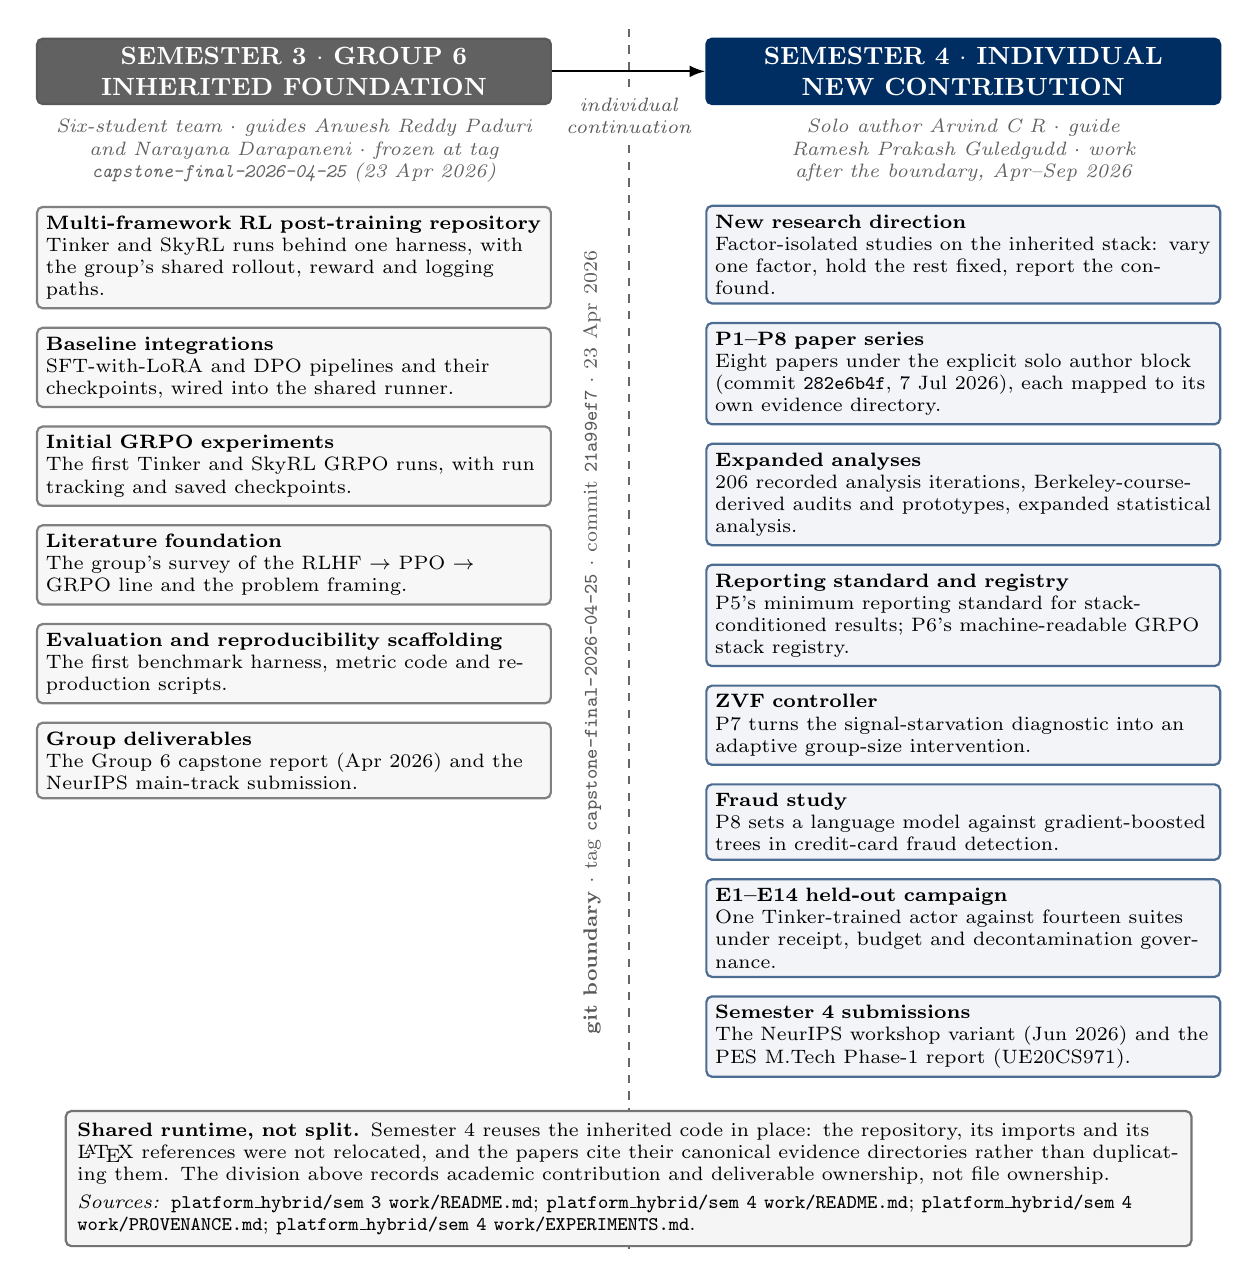
\begin{tikzpicture}

% ============================ column headers ============================
\node[hdrL, anchor=north] (hL) at (-4.25,0)
  {SEMESTER 3 $\cdot$ GROUP 6\\INHERITED FOUNDATION};
\node[hdrR, anchor=north] (hR) at ( 4.25,0)
  {SEMESTER 4 $\cdot$ INDIVIDUAL\\NEW CONTRIBUTION};

\node[sub, below=1.4mm of hL] (sL)
  {Six-student team $\cdot$ guides Anwesh Reddy Paduri and Narayana Darapaneni
   $\cdot$ frozen at tag \texttt{capstone-final-2026-04-25} (23 Apr 2026)};
\node[sub, below=1.4mm of hR] (sR)
  {Solo author Arvind C R $\cdot$ guide Ramesh Prakash Guledgudd
   $\cdot$ work after the boundary, Apr--Sep 2026};

% ============================ left column: inherited ====================
\node[itL, below=2.6mm of sL] (L1)
  {\textbf{Multi-framework RL post-training repository}\\Tinker and SkyRL runs behind
   one harness, with the group's shared rollout, reward and logging paths.};
\node[itL, below=2.2mm of L1] (L2)
  {\textbf{Baseline integrations}\\SFT-with-LoRA and DPO pipelines and their
   checkpoints, wired into the shared runner.};
\node[itL, below=2.2mm of L2] (L3)
  {\textbf{Initial GRPO experiments}\\The first Tinker and SkyRL GRPO runs, with run
   tracking and saved checkpoints.};
\node[itL, below=2.2mm of L3] (L4)
  {\textbf{Literature foundation}\\The group's survey of the
   RLHF $\rightarrow$ PPO $\rightarrow$ GRPO line and the problem framing.};
\node[itL, below=2.2mm of L4] (L5)
  {\textbf{Evaluation and reproducibility scaffolding}\\The first benchmark harness,
   metric code and reproduction scripts.};
\node[itL, below=2.2mm of L5] (L6)
  {\textbf{Group deliverables}\\The Group 6 capstone report (Apr 2026) and the
   NeurIPS main-track submission.};

% ============================ right column: individual ==================
\node[itR, below=2.6mm of sR] (R1)
  {\textbf{New research direction}\\Factor-isolated studies on the inherited stack:
   vary one factor, hold the rest fixed, report the confound.};
\node[itR, below=2.2mm of R1] (R2)
  {\textbf{P1--P8 paper series}\\Eight papers under the explicit solo author block
   (commit \texttt{282e6b4f}, 7 Jul 2026), each mapped to its own evidence directory.};
\node[itR, below=2.2mm of R2] (R3)
  {\textbf{Expanded analyses}\\206 recorded analysis iterations, Berkeley-course-derived
   audits and prototypes, expanded statistical analysis.};
\node[itR, below=2.2mm of R3] (R4)
  {\textbf{Reporting standard and registry}\\P5's minimum reporting standard for
   stack-conditioned results; P6's machine-readable GRPO stack registry.};
\node[itR, below=2.2mm of R4] (R5)
  {\textbf{ZVF controller}\\P7 turns the signal-starvation diagnostic into an adaptive
   group-size intervention.};
\node[itR, below=2.2mm of R5] (R6)
  {\textbf{Fraud study}\\P8 sets a language model against gradient-boosted trees in
   credit-card fraud detection.};
\node[itR, below=2.2mm of R6] (R7)
  {\textbf{E1--E14 held-out campaign}\\One Tinker-trained actor against fourteen suites
   under receipt, budget and decontamination governance.};
\node[itR, below=2.2mm of R7] (R8)
  {\textbf{Semester 4 submissions}\\The NeurIPS workshop variant (Jun 2026) and the
   PES M.Tech Phase-1 report (UE20CS971).};

% ============================ footer band ===============================
\node[fit=(L6)(R8), inner sep=0pt] (lowest) {};
\node[foot, below=4.0mm of lowest] (FOOT)
  {\textbf{Shared runtime, not split.} Semester 4 reuses the inherited code in place:
   the repository, its imports and its \LaTeX\ references were not relocated, and the
   papers cite their canonical evidence directories rather than duplicating them. The
   division above records academic contribution and deliverable ownership, not file
   ownership.\\[2pt]
   \textit{Sources:} \texttt{platform\_hybrid/sem 3 work/README.md};
   \texttt{platform\_hybrid/sem 4 work/README.md};
   \texttt{platform\_hybrid/sem 4 work/PROVENANCE.md};
   \texttt{platform\_hybrid/sem 4 work/EXPERIMENTS.md}.};

% ============================ boundary ==================================
\begin{scope}[on background layer]
  \node[fit=(hL)(hR)(FOOT), inner sep=3pt, draw=none, fill=none] (ALL) {};
  \draw[bnd] (ALL.north) -- (ALL.south);
\end{scope}

\node[rotate=90, font=\scriptsize, text=black!65, inner sep=1pt, align=center]
  at ($(ALL.north)!0.5!(ALL.south) + (-0.46,0)$)
  {\textbf{git boundary} $\cdot$ tag \texttt{capstone-final-2026-04-25}
   $\cdot$ commit \texttt{21a99ef7} $\cdot$ 23 Apr 2026};

% ============================ handover arrow ============================
\draw[ar] (hL.east) -- (hR.west);
\node[hdlbl] at ($(hL.east)!0.5!(hR.west) + (0,-0.56)$) {individual continuation};

\end{tikzpicture}
\end{document}
